\section{Ergebnisse}

Um einen guten Klassfizierer zu bekommen waren einige Trainingsdurchläufe notwendig. Zum testen der Klassifizierer wurden diese auf einen Validierungs-Datensatz angewandt. Die ersten Klassifizierer haben dabei nur minimal bessere Ergebnisse als der Zufall geliefert. Durch verschiedene Anpassungen, die in Kapitel~\ref{training} näher erläutert wurden, konnten schließlich besser Ergebnisse erreicht werden. Einige ausgewählte Ergebnisse werden in Abbildung~\ref{fig:roc} als ROC-Kurve dargestellt. Jede Kurve steht für einen ausgewählten Klassifizierer und die entsprechende Anwendung auf den Validierungs-Datensatz. Wie man gut erkennen kann verlaufen zwei der Kurven nahe der Diagonalen. Diese zwei Klassifikatoren (2018-03-12\_22-04-38 und 2018-03-12\_22-17-46) liefern somit keine guten Ergebnisse und sind nur etwas besser als hätten wir eine zufällige Entscheidung gefällt. Gute Klassifikatoren verlaufen in der ROC-Kurve links oben und sind in diesem Fall 2018-03-10\_19-16-32, 2018-03-09\_21-34-4 und 2018-04-13\_20-38-20. Die anderen Klassifikatoren können auf den ersten Blick als in Ordnung eingestuft werden.

\begin{figure}[htb!]
	\begin{center}
		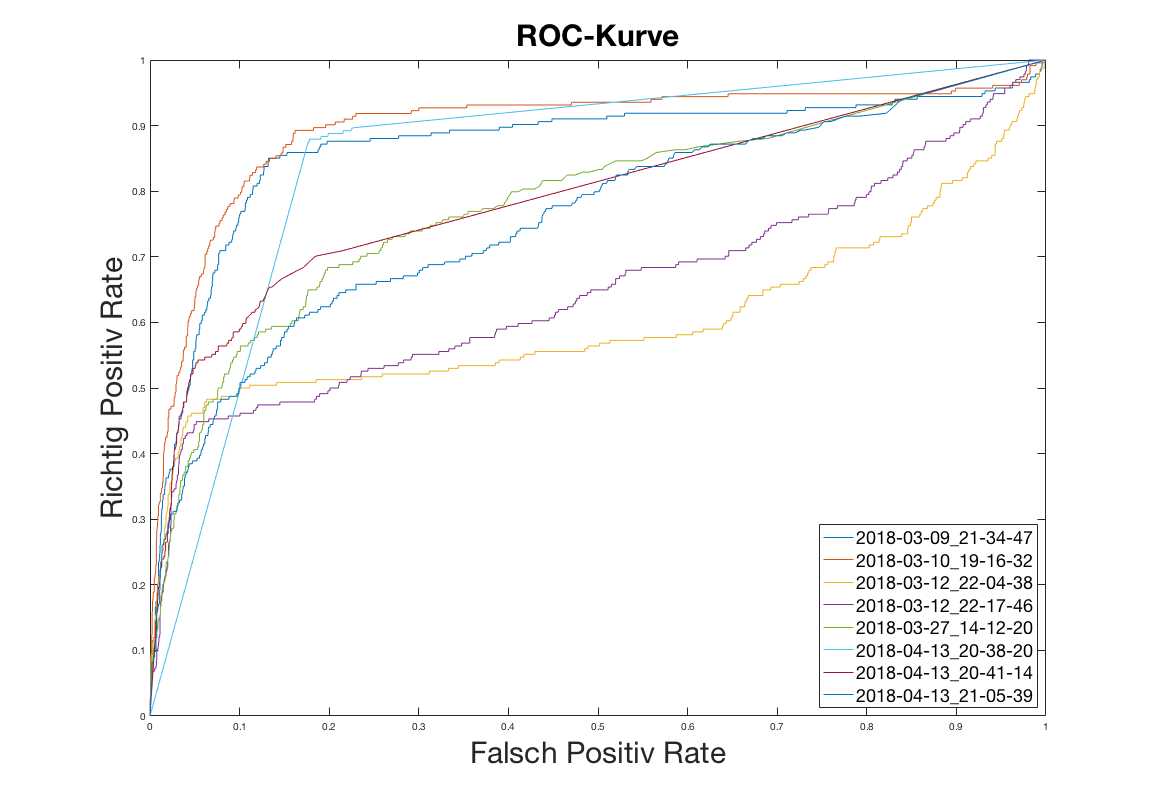
\includegraphics[width=\textwidth]{./pics/evaluation/roc_analysis.png}
		\caption{ROC-Kurven einiger trainierter Klassifizierer, angewandt auf den Validierungs-Datensatz.}
		\label{fig:roc}
    \end{center}
\end{figure}

Um die ROC-Kurve nicht optisch zu evaluieren zeigt Tabelle~\ref{tab:auc} die Klassifikatoren aus Abbildung~\ref{fig:roc} zusammen mit ihrer berechneten \textit{area under the curve} (AUC). Es ist deutlich zu erkennen, dass die kurven die links oben verlaufen gleichzeitig eine höhere AUC aufweisen. Somit ist der Klassifikator 2018-03-12\_22-04-38 mit einem AUC von $0.6$ der Schlechteste und nur leicht besser als eine Zufallsvorhersage. Der Klassifikator 2018-03-10\_19-16-32 hingegen ist mit einem AUC von 0.9 der in diesem Fall Beste. 

\begin{table}[htb!]
\begin{center}
\begin{tabular}{ll}
	\toprule
 	Klassifikator  & AUC\\
	\midrule
  	2018-03-09\_21-34-47 &   $0.87$\\
    2018-03-10\_19-16-32 &   $0.90$\\
    2018-03-12\_22-04-38 &   $0.60$\\
    2018-03-12\_22-17-46 &   $0.65$\\
    2018-03-27\_14-12-20 &   $0.78$\\
    2018-04-13\_20-38-20 &   $0.86$\\
    2018-04-13\_20-41-14 &   $0.79$\\
    2018-04-13\_21-05-39 &   $0.75$\\
 \bottomrule
 \end{tabular}
 \end{center}
  \caption{ROC-AUC Ergebnisse einiger trainierten Klassifikatoren}
 \label{tab:auc}
 \end{table}
 
Da wir bei der Hautkrebs-Erkennung noch ein paar Sonderanforderungen an den Klassifikator haben und einen sehr unausgeglichenen Datensatz verwendeten, entschieden wir uns die zwei Klassifikatoren mit der höchsten AUC (2018-03-10\_19-16-32 und 2018-03-09\_21-34-47) noch genauer zu Evaluieren. Unser Klassifizierer soll am Ende  eine hohe Vorhersagegenauigkeit haben, allerdings sollten nicht zu viele wirklich positive Ergebnisse (maligne) als negativ (benigne) klassifiziert werden. Unter Berücksichtigung wurden für dieses zwei Klassifikatoren noch weitere Qualitätsmaßstäbe berechnet. Tabelle~\ref{tab:scores} zeigt die verschiedenen Qualitätsmaßstäbe,  die schon in Kapitel~\ref{analysemethoden} vorgestellt wurden. Wie man der Tabelle gut entnehmen kann ist Klassifikator 2018-03-10\_19-16-32 in nahezu allen belangen besser als 2018-03-09\_21-34-47. Einzig und allein in der Spezifität weißt er einen minimal schlechteren Wert auf.

\begin{table}[htb!]
\begin{center}
\begin{tabular}{lllllllllll}
	\toprule
 	Klassifikator  & TP & FN & TN & FP & MCC & F2 & Acc & Sens & Spez\\
	\midrule
	2018-03-09\_21-34-47 & $119$ &	$115$ &	$2406$ &	$113$ &	$0.47$ &	$0.51$&	$0.92$ &	$0.51$ & $0.96$\\
    2018-03-10\_19-16-32 & $142$&	$91$ &	$2406$ &	$114$ &	$0.54$ 	&$0.60$	&$0.93$	&$0.61$&	$0.95$ \\
 \bottomrule
 \end{tabular}
 \end{center}
  \caption{Scores der zwei besten Klassifizierer: TP = True Positives, FN = False Negatives, TN = True Negatives, FP = False Positives, MCC = Matthews Correlation Coefficient, F2 = F2-Score, Acc = Genauigkeit, Sens = Sensitivität und Spez = Spezifität }
 \label{tab:scores}
 \end{table}
 
 Da unser Klassifikator maligne Hautläsionen auch wirklich als solche Erkennen soll präferieren wir in diesem Fall die wenigen Falsch negativen und die mehr wirklich positive Ergebnisse. Dabei wurde sogar trotzdem nur ein negatives Ergebnis mehr fälschlicherweise als positiv (maligne) eingeordnet. Aufgrund dieser Evaluierung schlossen wir, dass der Klassifizierer mit der höheren AUC, Genauigkeit und Sensitivität, sowie einem  höherem MCC und F2-Score unser Problem der Hautkrebserkennung besser lösen kann. Eine etwas geringere Spezifität nehmen wir hierbei in Kauf, wobei diese so gering ist, dass es sich auch um eine Zufallserscheinung handeln könnte.
 
Obwohl der Klassifizierer insgesamt schon gute Vorhersagen macht, werden die Ergebnisse durch die hohe Spezifität von 95\% etwas verfälscht. Mit einer Sensitivität von $0.6$ würden wir nämlich nur $60\%$ aller malignen Hautläsionen auch als wirklich maligne klassifizieren. Im Umkehrschluss heißt das, dass vier von zehn potentielle malignen Hautläsionen unerkannt bleiben. Da diese Sensitivität noch zu nah an einer Zufallsklassifizierung liegt, schauten wir uns die Ergebnisse des Neuronalen Netzes des Klassifikators 2018-03-10\_19-16-32 noch einmal genauer an, da dieser in der vorherigen Evaluierung die besten Werte aufgewiesen hat. Das Ergebnis des Neuronalen Netz ist ein Score, der zwischen null und eins liegt. Ein Score über $0.5$ klassifiziert eine Hautläsion als maligne, ist er kleiner als $0.5$ als benigne. Um den Klassifizierer nun weiter in die von uns gewünschte Richtung zu lenken verschoben wir die Entscheidungsschranke (Threshold) und schauten wie sich diese Verschiebung auf die Klassifikation des Validierungs-Datensatzes auswirkte. Diese Auswirkung auf die verschiedenen Qualitätsmaßstäbe wird in Abbildung~\ref{fig:threshold} dargestellt. 

\begin{figure}[htb!]
	\begin{center}
		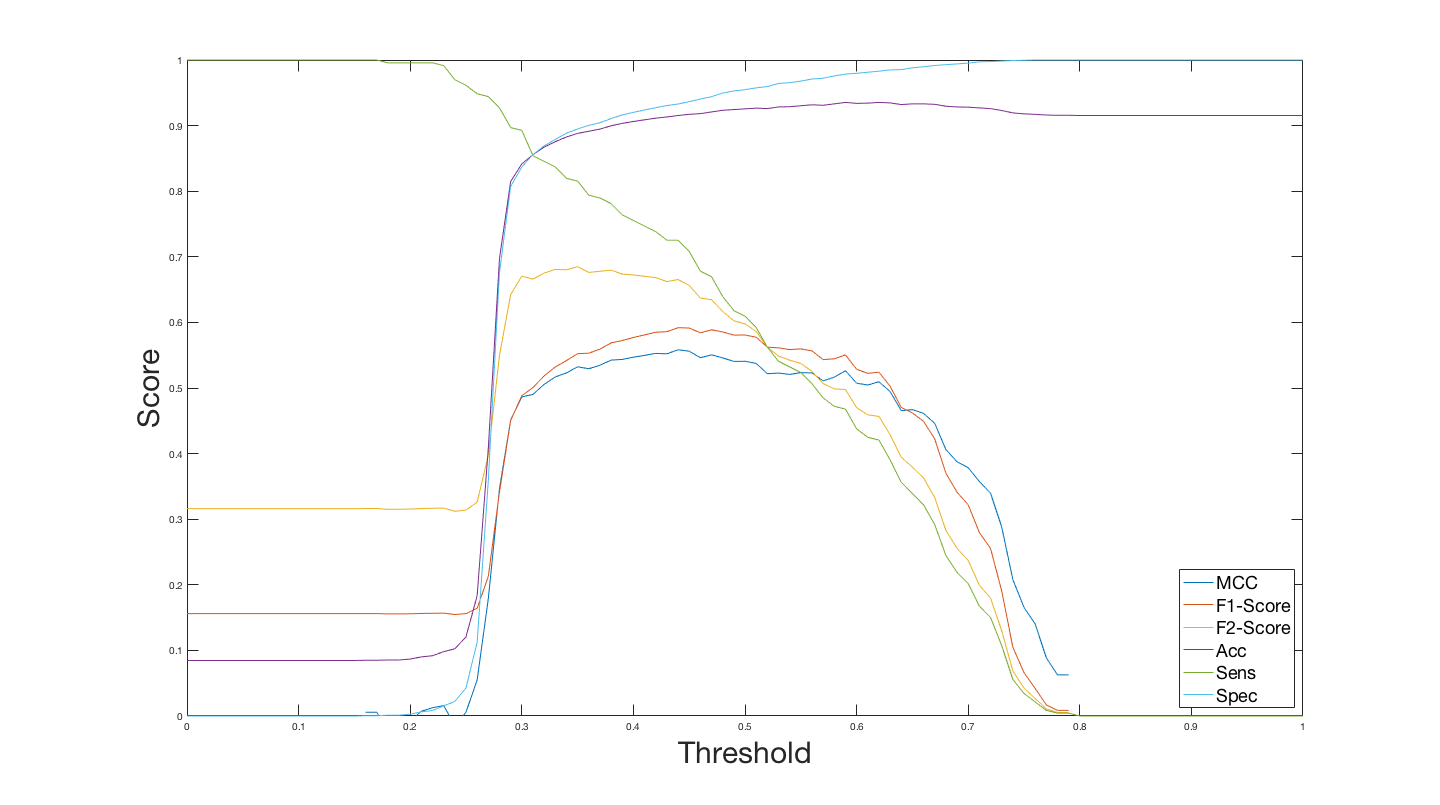
\includegraphics[width=\textwidth]{./pics/evaluation/treshold.png}
		\caption{Score-Threshold Abhängigkeit}
		\label{fig:threshold}
    \end{center}
\end{figure}

Wie man der Abbildung entnehmen kann, gibt es einen Bereich zwischen $0.3$ und $0.6$ in der der MCC und F2-Score gute Werte aufweisen. Da der F2-Score die falsch-negativen noch stärker bestraft konzentrierten wir uns hier mehr auf diesen Qualitätsmaßstab. Außerdem wollten wir eine möglichst hohe Sensitivität erreichen. Der F2-Score weist im Bereich $0.3$ und $0.45$ seine höchsten Werte auf, wobei der kleinste Threshold gleichzeitig die höchste Sensitivität liefert. Es wäre also naheliegend gewesen einfach diesen Wert zu nehmen. Da die Spezifität zwischen dem Threshold $0.25$ und $0.3$ rapide ansteigt sollte allerdings ein gewisser Abstand zu diesem Bereich gewahrt werden. 

Abbildung~\ref{fig:verteilung} zeigt die Verteilung der Scores des Validierung-Datensatz, der durch 2018-03-10\_19-16-32 klassifiziert wurde. Sie zeigt noch einmal deutlicher, dass die meisten benignen Beispiele zwischen einen Score zwischen $0.2$ und $0.3$ aufweisen. Somit entschieden wir uns den Threshold von den ursprünglichen $0.5$ auf $0.35$ herunterzusetzen. Damit halten wir genug Abstand von der extremen Änderung der Spezifität, klassifizieren deutlich mehr maligne Beispiele richtig ohne zu viele Fehler bei den negativen Beispielen zu machen. 

\begin{figure}[htb!]
	\begin{center}
		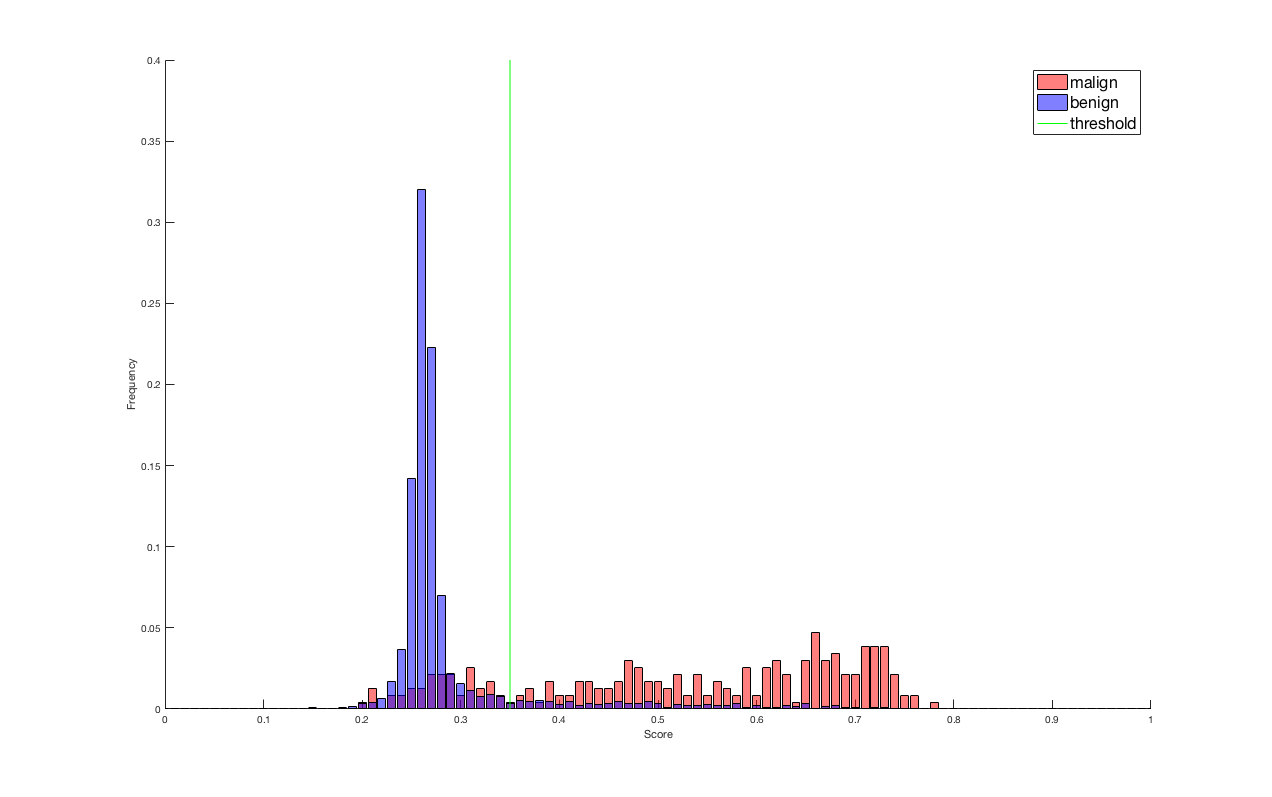
\includegraphics[width=\textwidth]{./pics/threshold/score_threshold.png}
		\caption{Verteilung unserer Ergebnisse des Validierungs-Datensatzes. Maligne Beispiele werden in rot dargestellt, benigne in blau.}
		\label{fig:verteilung}
    \end{center}
\end{figure}


Durch diese nun sensitivere Klassifizierung erhielten wir schließlich die Werte wie sie in Tabelle~\ref{tab:final_scores} gelistet sind. Die Sensitivität konnten wir durch die Verschiebung des Thresholds von $0.61$ auf $0.81$ erhöhen. Es werden also nur noch zwei von zehn maligne Hautläsionen als fälschlicherweise als benigne klassifiziert. Dabei nahmen wir eine Verringerung der Spezifität von $0.95$ auf $0.89$ in kauf. Es wird also etwa jede zehnte benigne Hautläsion falsch als maligne klassifiziert. Die Genauigkeit verringerte sich dabei von $93\%$ auf $0.89\%$, allerdings erhöhten wir den F2-Score von $0.6$ auf $0.68$, der bei einem unausgeglichenen Datensatz höher zu gewichten ist als die Gesamtgenauigkeit.

\begin{table}[htb!]
\begin{center}
\begin{tabular}{lllllllllll}
	\toprule
 	Threshold  & TP & FN & TN & FP & MCC & F2 & Acc & Sens & Spez\\
	\midrule
    $0.5$ & $142$&	$91$ &	$2406$ &	$114$ &	$0.54$ 	&$0.60$	&$0.93$	&$0.61$&	$0.95$ \\
	$0.35$ & $190$ & $43$ &	$2255$ &	$265$ &	$0.55$ &	$0.68$&	$0.89$ &	$0.81$ & $0.89$\\
 \bottomrule
 \end{tabular}
 \end{center}
  \caption{Scores des Klassifikators mit dem Threshold bei $0.35$}
 \label{tab:final_scores}
 \end{table}

\todo{Parameter für besten Trainingsdurchlauf}
\todo{Anwendung auf Test und finaler Klassifikator}